This chapter describes the methods developed to connect a real,
assembly-resolved U.S. spent fuel inventory to an accelerator-driven burner
within a single fuel cycle simulation. The work required building two new
facility archetypes for \Cyclus, \texttt{us\_inventory} and \texttt{ads}, and
assembling them together with existing fuel cycle facilities into complete
transmutation scenarios. The chapter sets out the overall modeling approach,
the language and software framework in which the archetypes are implemented,
the design and data behind each archetype in turn, and finally the specific
fuel cycle configurations and simulation runs used to generate the results
presented in Chapter~\ref{ch:results}.

\section{Overview of the Simulation Approach}
\label{sec:method-overview}

The simulations in this work are performed with \Cyclus, the agent-based
nuclear fuel cycle simulator introduced in Chapter~\ref{ch:background}. Two
facility archetypes were developed within the \texttt{einstein} archetype
library: \texttt{us\_inventory}, which represents the United States inventory of
\gls{UNF} at the resolution of individual assemblies, and \texttt{ads}, which
represents an accelerator-driven subcritical burner. These are combined with
facilities from the \Cycamore library, \texttt{Separations} to partition
discharged fuel into product and waste streams, \texttt{Mixer} to blend separated
streams into a burner feed, and \texttt{Sink} to receive final waste, to form a
complete transmutation fuel cycle. The two variants of this cycle used in this
work, once-through and recycling, are shown in
Figures~\ref{fig:flowsheet-oncethrough} and~\ref{fig:flowsheet-recycle} in
Section~\ref{subsec:scenario-flowsheet}.

The remainder of this chapter describes each archetype in turn, 
\texttt{us\_inventory} in Section~\ref{sec:us-inventory-archetype} and
\texttt{ads} in Section~\ref{sec:ads-archetype}, and then defines the specific
scenarios built from them in Section~\ref{sec:simulation-scenarios}.

All scenarios share a common set of simulation settings. Time advances in
monthly steps of \(30.4375~\mathrm{d}\), beginning in January~2025, over a
horizon of either 30 years (360 steps) or 100 years (1200 steps). Radioactive
decay is enabled at the simulation level through the \Cyclus control block with
decay set to \texttt{lazy}, so that material compositions are decayed on demand
over the multi-decade horizon rather than at every time step
\cite{huff_fundamental_2016}. The full set of runs and the parameters for each scenario are given in
Section~\ref{sec:simulation-scenarios}.

%%%%%%%%%%%%%%%%%%%%%%%%%%%%%%%%%%%%%%%%%%%%%%%%%%%%%%%%%%%%%%%%%%%%%%%%%%%%%%%%%%%%%%%%%%%%%%%%%%%%%%%%%%%%%%%%%%%%%%%%%%%%%%%%%
%%%%%%%%%%%%%%%%%%%%%%%%%%%%%%%%%%%%%%%%%%%%%%%%%%%%%%%%%%%%%%%%%%%%%%%%%%%%%%%%%%%%%%%%%%%%%%%%%%%%%%%%%%%%%%%%%%%%%%%%%%%%%%%%%
%%%%%%%%%%%%%%%%%%%%%%%%%%%%%%%%%%%%%%%%%%%%%%%%%%%%%%%%%%%%%%%%%%%%%%%%%%%%%%%%%%%%%%%%%%%%%%%%%%%%%%%%%%%%%%%%%%%%%%%%%%%%%%%%%
\section{Implementation within \Cyclus}
\label{sec:method-implementation}

Both archetypes are written in C++, the language of the \Cyclus kernel itself
\cite{huff_fundamental_2016}. Each is implemented as a header and
implementation file pair within the \texttt{einstein} archetype library,
under a shared \texttt{einstein} namespace, following the same structure and
conventions as the standard \Cycamore library on which it is
modeled \cite{carlsen_cycamore_2014}. The library is maintained as an
open-source repository on GitHub\footnote{\url{https://github.com/arfc/einstein}},
alongside the \Cyclus kernel\footnote{\url{https://github.com/cyclus/cyclus}},
and the \Cycamore archetypes\footnote{\url{https://github.com/cyclus/cycamore}},
and is compiled into a dynamically loadable archetype library that the
\Cyclus kernel loads at runtime according to the archetypes named in a
simulation's input file.

An archetype becomes a \Cyclus facility by inheriting from the framework's
base classes rather than by reimplementing simulation infrastructure. The
\texttt{us\_inventory} archetype derives from \texttt{cyclus::Facility}, which
in turn derives from \texttt{cyclus::Agent}, and additionally from
\texttt{cyclus::toolkit::CommodityProducer} so that it is recognized as a
producer of a configured output commodity; the \texttt{ads} archetype derives
from \texttt{cyclus::Facility} alone. A single header, \texttt{cyclus.h},
exposes the kernel interface used throughout: the simulation
\texttt{Context}, the \texttt{Material} and \texttt{Composition} resource
types, the resource exchange objects through which facilities bid on and trade
material, and the toolkit utilities on which the archetypes rely. Inheriting
from these classes places each archetype directly into the agent-based
scheduling and \gls{DRE} machinery described in Chapter~\ref{ch:background},
so that development can focus on facility behavior rather than on the
mechanics of the simulation loop.

The remaining connective code is generated automatically by the \Cyclus
preprocessor, \texttt{cycpp}, which processes \texttt{\#pragma cyclus}
annotations embedded in the source. Persistent state is declared by marking a
member variable with \texttt{\#pragma cyclus var}, which records the
information the kernel needs to validate that variable against the input
schema, write it to and restore it from the simulation database, and copy it
when an agent is cloned. Companion directives request the default generated
implementations of these operations and attach human-readable documentation to
the archetype. This arrangement keeps the input specification, database schema,
and internal state of each archetype consistent without handwritten
boilerplate, so that the source files contain primarily the physical and
logical behavior of the inventory and burner models that the remainder of this
chapter describes.

%%%%%%%%%%%%%%%%%%%%%%%%%%%%%%%%%%%%%%%%%%%%%%%%%%%%%%%%%%%%%%%%%%%%%%%%%%%%%%%%%%%%%%%%%%%%%%%%%%%%%%%%%%%%%%%%%%%%%%%%%%%%%%%%%
%%%%%%%%%%%%%%%%%%%%%%%%%%%%%%%%%%%%%%%%%%%%%%%%%%%%%%%%%%%%%%%%%%%%%%%%%%%%%%%%%%%%%%%%%%%%%%%%%%%%%%%%%%%%%%%%%%%%%%%%%%%%%%%%%
%%%%%%%%%%%%%%%%%%%%%%%%%%%%%%%%%%%%%%%%%%%%%%%%%%%%%%%%%%%%%%%%%%%%%%%%%%%%%%%%%%%%%%%%%%%%%%%%%%%%%%%%%%%%%%%%%%%%%%%%%%%%%%%%%
\section{The \texttt{us\_inventory} Archetype}
\label{sec:us-inventory-archetype}

The \texttt{us\_inventory} archetype represents the existing U.S. \gls{UNF}
inventory as an active material supplier. Rather than collapsing the national
inventory into a single resource with a prescribed mass and representative
composition, it preserves individual assembly records, because the U.S.
inventory is heterogeneous and the order in which assemblies are selected changes
the mass and isotopic composition delivered to downstream facilities.

Each assembly is stored as a separate inventory assembly with its own mass, operating
history, storage information, composition, and geographic provenance. During a
simulation the facility answers material requests through the \Cyclus \gls{DRE}
(Chapter~\ref{ch:background}) and selects an eligible assembly according to a
user-specified policy, reducing that assembly's mass and the total inventory as
material is supplied. It inherits from \texttt{cyclus::Facility} and
\texttt{cyclus::toolkit::CommodityProducer}, so it acts as both a facility agent
and a producer of a configured output commodity. The facility performs no
scheduled action each time step; all of its behavior is triggered either when the
input data are loaded at initialization or when it participates in resource
exchange. The overall structure of the archetype is illustrated in
Figure~\ref{fig:usinv-structure}.


\begin{figure}[h!]
\centering
\resizebox{0.95\textwidth}{!}{%
\begin{tikzpicture}[
    font=\rmfamily,
    box/.style={
        draw,
        rounded corners=12pt,
        line width=0.9pt,
        minimum width=8.2cm,
        minimum height=3.2cm,
        fill=blue!15,
        align=center
    },
    %, arrow styles (edit colors here), 
    a1/.style={->, line width=1pt, blue!40!black},
    a2/.style={->, line width=1pt, blue!98!black},
    a3/.style={->, line width=1pt, cyan!85!black},
    afinal/.style={->, line width=1pt, teal!80!black},
    %, consistent label style, 
    lab/.style={font=\small, align=center}
]

% Main box
\node[box] (inv) {\LARGE U.S. Inventory};

%, geometry controls, 
\def\arrowlen{6}        % arrow length to the right
\def\dy{0.6}            % equal spacing between arrows
\def\yone{0.9}          % top arrow offset (controls stack position)

% First three equally spaced arrows
\draw[a1] (inv.east) ++(0,\yone) -- ++(\arrowlen,0)
    node[midway, above, lab] {PWR, Init\_Enr=3.8\%, BU=41919};

\draw[a2] (inv.east) ++(0,\yone-\dy) -- ++(\arrowlen,0)
    node[midway, above, lab] {PWR, Init\_Enr=4.2\%, BU=43597};

\draw[a3] (inv.east) ++(0,\yone-2*\dy) -- ++(\arrowlen,0)
    node[midway, above, lab] {BWR, Init\_Enr=2.19\%, BU=6237};

% Three short vertical bars marking additional assemblies.
% They are drawn directly in the main picture to avoid nesting a tikzpicture.
\coordinate (continuation) at
    ($(inv.east)+(0.5*\arrowlen,\yone-2.5*\dy)$);
\draw[line width=1.1pt, teal!85!black]
    ($(continuation)+(0,0.19)$) -- ($(continuation)+(0,0.11)$);
\draw[line width=1.1pt, teal!80!black]
    ($(continuation)+(0,0.05)$) -- ($(continuation)+(0,-0.03)$);
\draw[line width=1.1pt, teal!70!black]
    ($(continuation)+(0,-0.10)$) -- ($(continuation)+(0,-0.18)$);

% Last arrow (different color) + label
\draw[afinal] (inv.east) ++(0,\yone-3.6*\dy) -- ++(\arrowlen,0)
    node[midway, above, lab] {$N$ assemblies in the nation};

\end{tikzpicture}
}
\caption{Structure of the U.S. Inventory module based on the STANDARDS~5.0.1 dataset. Representative PWR and BWR assemblies are identified by their initial enrichment, burnup, and isotopic composition, and the module retains all assemblies in the national spent fuel inventory.}
\label{fig:usinv-structure}
\end{figure}

\subsection{Purpose and Assembly-Level Data Source}
\label{subsec:us-inventory-data}

The source data are assembly-level records derived from \gls{STANDARDS}~5.0.1,
which associates individual U.S. spent fuel assemblies with facility, storage,
irradiation history, and calculated isotopic information. This level of detail
distinguishes assemblies that would otherwise be represented using an average
composition for a facility or for the national inventory
\cite{peterson_additional_2017,abdelkawy_summary_2025}.

For the simulations in this thesis, the \gls{STANDARDS} data were provided as a
directory of 75 line-delimited files, one per represented facility. The file
count is not hard-coded: the \texttt{data\_dir} parameter names a directory, and
every file whose name ends in \texttt{.txt} or contains \texttt{.jsonl} is read,
so the archetype can run on a subset of the database without recompilation.

Each nonempty line is one assembly record, converted into assembly metadata and a
nuclide mass map. Because the export wraps each dictionary-like record in an outer
JSON string, a purpose-built parser removes that wrapper and accepts both single-
and double-quoted strings. It reads the facility name, storage location name,
assembly identifier, storage type, discharge year, initial enrichment, maximum
burnup, initial uranium mass, and a dictionary of nuclide masses in grams.
Unrecognized fields are ignored, and records with no nonzero composition are
skipped.

The nuclide names are converted to the integer \texttt{ZZAAAM} identifiers used by
\Cyclus and assembled into a \texttt{cyclus::Composition}; the total assembly mass
is converted from grams to kilograms and stored with the record. Each assembly is
held in an \texttt{assembly} structure, summarized in Table~\ref{tab:usinv-bin}.

\begin{table}[h!]
    \centering
    \caption{Fields stored in each \texttt{assembly} structure.}
    \label{tab:usinv-bin}
    \begin{tabular}{p{0.34\textwidth} p{0.58\textwidth}}
        \hline
        \textbf{Field} & \textbf{Description} \\
        \hline
        Assembly\_ID          & Original database assembly identifier. \\
        Facility, location    & Source facility and storage location names. \\
        Storage type          & Wet or dry storage. \\
        Available mass        & Current material mass, in kilograms. \\
        Discharge year        & Year the assembly was discharged. \\
        Maximum burnup        & Reported maximum burnup. \\
        Initial enrichment    & Initial uranium enrichment. \\
        Initial uranium mass  & Initial mass of uranium. \\
        Derived fractions     & Fissile, plutonium, and minor actinide
        mass fractions. \\
        Coordinates           & Latitude and longitude of the source facility. \\
        Composition           & Complete \Cyclus composition of the assembly. \\
        \hline
    \end{tabular}
\end{table}

Because the original identifier is not unique across the dataset, the archetype
builds an internal key from the facility name, storage location, original
identifier, and load position, stored in \texttt{assembly\_id}; the raw value is
kept in \texttt{orig\_id}. Each assembly's available mass starts as the sum of its
reported nuclide masses, and a running total tracks the material remaining in the
facility.

Three composition fractions used by the selection policies are computed once at
load time. For assembly \(a\) with total mass \(m_a\) and nuclide mass
\(m_{i,a}\) for nuclide \(i\), the fissile mass fraction is

\begin{equation}
    f_{\mathrm{fissile},a}
    =
    \frac{
        m_{^{233}\mathrm{U},a}
        + m_{^{235}\mathrm{U},a}
        + m_{^{239}\mathrm{Pu},a}
        + m_{^{241}\mathrm{Pu},a}
    }{m_a},
    \label{eq:usinv-fissile-fraction}
\end{equation}

where the numerator sums the masses of \({}^{233}\mathrm{U}\),
\({}^{235}\mathrm{U}\), \({}^{239}\mathrm{Pu}\), and \({}^{241}\mathrm{Pu}\) in
assembly \(a\), and \(m_a\) is its total mass. The total plutonium mass fraction
is

\begin{equation}
    f_{\mathrm{Pu},a}
    =
    \frac{\displaystyle\sum_{i \in \mathrm{Pu}}m_{i,a}}{m_a},
    \label{eq:usinv-pu-fraction}
\end{equation}

where the sum runs over all plutonium isotopes present in assembly \(a\). The
minor actinide mass fraction is

\begin{equation}
    f_{\mathrm{MA},a}
    =
    \frac{
        \displaystyle
        \sum_{i \in \mathrm{Np}}m_{i,a}
        + \sum_{i \in \mathrm{Am}}m_{i,a}
        + \sum_{i \in \mathrm{Cm}}m_{i,a}
    }{m_a},
    \label{eq:usinv-ma-fraction}
\end{equation}

where each sum runs over all isotopes of neptunium, americium, or curium in
assembly \(a\). These fractions are precomputed so the selection policies need not
traverse the full nuclide composition on every request.

The required inputs are the output commodity, \texttt{outcommod}, and the
assembly data directory, \texttt{data\_dir}. An optional maximum throughput,
\texttt{throughput\_kg}, in kilograms per time step, is effectively unlimited by
default but can be reduced to represent a constraint on inventory retrieval,
transportation, or processing.

\subsection{Assembly Provenance and Geographic Coordinates}
\label{subsec:us-inventory-provenance}

Preserving assembly provenance connects inventory selection results to later
transportation, siting, and infrastructure analyses. The \gls{STANDARDS} records
identify each assembly's facility and storage location but not its coordinates,
so an optional SQLite database associates a facility name with latitude and
longitude.

The database path is supplied through \texttt{coordinates\_file}. If it is empty,
the archetype still runs but every assembly keeps the default pair \((0,0)\). When a
database is provided, it is opened read-only and queried for the facility name,
taking an exact match where one exists and otherwise a prefix match. All
assemblies from a facility share one coordinate pair, cached after the first
lookup. If no entry matches, the archetype warns and leaves that facility at
\((0,0)\).

Every completed transfer is recorded in a custom \Cyclus output table,
\texttt{us\_inventorySupply}, with one row per supplied trade
(Table~\ref{tab:usinv-supply}). The transferred material separately carries the
composition built from the selected assembly, so a transaction can be traced to both
its source assembly and its material composition.

\begin{table}[h!]
    \centering
    \caption{Columns written to the \texttt{us\_inventorySupply} output table.}
    \label{tab:usinv-supply}
    \begin{tabular}{p{0.34\textwidth} p{0.58\textwidth}}
        \hline
        \textbf{Column} & \textbf{Description} \\
        \hline
        Agent ID          & Identifier of the supplying agent. \\
        Time              & Simulation time step of the transfer. \\
        Facility          & Source facility name. \\
        Storage location  & Source storage location name. \\
        Storage type      & Wet or dry storage. \\
        Assembly ID       & Original assembly identifier. \\
        Initial uranium   & Initial uranium mass of the assembly. \\
        Latitude, longitude & Coordinates of the source facility. \\
        Quantity          & Mass supplied in the trade. \\
        Selection policy  & Policy in force for the simulation. \\
        \hline
    \end{tabular}
\end{table}

\subsection{Assembly Selection Policies}
\label{subsec:us-inventory-policies}

The archetype's principal methodological feature is its ability to choose among
individual assemblies by explicit ranking policies. In resource exchange the
solver decides which offers and requests match, but the supplier still chooses
which physical resource fulfills an accepted trade; \texttt{us\_inventory} uses
this selection step to model different assumptions about access to the legacy
inventory.

The policy is set through \texttt{selection\_policy} and checked at
initialization, where an unrecognized value stops the simulation with a
descriptive input error. For each trade the archetype scans the eligible assemblies and
keeps the one ranked highest under the active criterion, skipping empty assemblies and
assemblies without a valid composition. Table~\ref{tab:usinv-selection-policies} lists
the 15 policies.

\begin{table}[h!]
    \centering
    \caption{Assembly selection policies implemented by the
    \texttt{us\_inventory} archetype. Each policy ranks the eligible
    assemblies before a trade is fulfilled.}
    \label{tab:usinv-selection-policies}
    \begin{tabular}{p{0.34\textwidth} p{0.58\textwidth}}
        \hline
        \textbf{Policy} & \textbf{Assembly selected} \\
        \hline
        \texttt{first}                    & First eligible assembly in the database. \\
        \texttt{older}                    & Earliest discharge year. \\
        \texttt{newer}                    & Latest discharge year. \\
        \texttt{highest\_burnup}          & Largest reported maximum burnup. \\
        \texttt{lowest\_burnup}           & Smallest reported maximum burnup. \\
        \texttt{highest\_enrichment}      & Largest initial enrichment. \\
        \texttt{lowest\_enrichment}       & Smallest initial enrichment. \\
        \texttt{highest\_initial\_uranium}& Largest initial uranium mass. \\
        \texttt{lowest\_initial\_uranium} & Smallest initial uranium mass. \\
        \texttt{highest\_fissile}         & Largest fissile fraction
        (Eq.~\ref{eq:usinv-fissile-fraction}). \\
        \texttt{lowest\_fissile}          & Smallest fissile fraction. \\
        \texttt{highest\_plutonium}       & Largest plutonium fraction
        (Eq.~\ref{eq:usinv-pu-fraction}). \\
        \texttt{lowest\_plutonium}        & Smallest plutonium fraction. \\
        \texttt{highest\_minor\_actinide} & Largest minor actinide fraction
        (Eq.~\ref{eq:usinv-ma-fraction}). \\
        \texttt{lowest\_minor\_actinide}  & Smallest minor actinide fraction. \\
        \hline
    \end{tabular}
\end{table}

Ranking keeps the first eligible assembly as the initial candidate and replaces it
only when a later assembly is strictly better under the criterion, so ties retain their
load order priority.

Two optional inputs bias the pool toward a particular source.
\texttt{preferred\_facility} names a specific facility, and \texttt{storage\_type}
restricts the pool to \texttt{wet} or \texttt{dry} storage. These filters are
preferential rather than exclusive: the matching assemblies are searched first,
and if they cannot supply a trade the rest of the inventory is searched, with a
warning the first time this fallback occurs. This keeps the archetype consistent
with the \gls{DRE}, which expects a bidding facility to remain able to supply an
accepted trade.

Whether a request may be partially filled is governed by \texttt{allow\_partial}.
Selection first requires that an assembly cover the full requested mass; only if none
can, and \texttt{allow\_partial} is true, is a smaller quantity permitted.
Each accepted trade is drawn from a single assembly. The archetype does not combine
undersized assemblies, which preserves a one-to-one relationship between each trade
response and the assembly recorded in \texttt{us\_inventorySupply}.

\subsection{Material Bidding, Trading, and Accounting}
\label{subsec:us-inventory-accounting}

Bidding and trading are handled in two stages: the facility first advertises how
much material it can offer, and then, once trades are awarded, withdraws a
specific assembly for each one.

When there are requests on the output commodity, the facility bids. Because the
source filters are preferential, the whole remaining inventory is eligible, so the
facility can fall back to nonmatching assemblies. The compositions of the eligible
assemblies are combined into a single mass-weighted bid composition,

\begin{equation}
    \mathbf{x}_{\mathrm{bid}}
    =
    \frac{
        \displaystyle\sum_{a \in \mathcal{E}} m_a\,\vec{\mathbf{m}_a}
    }{
        \displaystyle\sum_{a \in \mathcal{E}} m_a
    },
    \label{eq:usinv-bid-composition}
\end{equation}

where \(\mathcal{E}\) is the set of eligible assemblies, \(m_a\) is the remaining mass of
assembly \(a\), and \(\vec(\mathbf{m}_a)\) is its vector of nuclide mass fractions. The
maximum mass offered is

\begin{equation}
    M_{\mathrm{offer}}
    =
    \min\!\left(
        M_{\mathrm{eligible}},\;
        M_{\mathrm{throughput}}
    \right),
    \label{eq:usinv-offer-capacity}
\end{equation}

where \(M_{\mathrm{eligible}} = \sum_{a \in \mathcal{E}} m_a\) is the total mass of
the eligible pool and \(M_{\mathrm{throughput}}\) is the configured
throughput per time step. This value enters the portfolio as a capacity
constraint. With partial fulfillment disabled, the archetype does not bid on a
request larger than it can offer.

The bid composition represents the available pool but does not replace
selection of the source assembly according to the active policy. After the
solver awards trades,
each one is matched to a source assembly by the procedure in
Section~\ref{subsec:us-inventory-policies}, so the material returned is built from
the selected assembly's composition, not the averaged bid composition.

Each accepted trade is limited by the requested quantity, the selected assembly's
remaining mass, and the throughput remaining in the step, and fulfillment stops
once the throughput or the inventory is exhausted. After each response the
archetype updates

\begin{align}
    m_{a,t+1}
    &= m_{a,t} - m_{\mathrm{supplied}},
    \label{eq:usinv-bin-update} \\
    M_{\mathrm{inv},t+1}
    &= M_{\mathrm{inv},t} - m_{\mathrm{supplied}},
    \label{eq:usinv-inv-update} \\
    R_{t+1}
    &= R_{t} - m_{\mathrm{supplied}},
    \label{eq:usinv-throughput-update}
\end{align}

where \(m_{a,t}\) is the available mass of the selected assembly \(a\),
\(M_{\mathrm{inv},t}\) is the total mass remaining in the facility, \(R_t\) is the
throughput remaining in the current step, and \(m_{\mathrm{supplied}}\) is the mass
delivered by the trade.

The remaining mass of each assembly is also persisted as archetype state, with
one value stored for every loaded assembly. Restarting from a checkpoint
reloads the assembly metadata
and compositions from the source files, overwrites their initial masses with the
persisted values, and rebuilds the inventory total from them. The simulation is
stopped if the number of persisted values does not match the number of loaded
assemblies, since that indicates the data directory changed after the checkpoint.

After each successful transaction the archetype appends a row to
\texttt{us\_inventorySupply}, giving a time-dependent history of which assemblies
were selected, where they originated, how much they supplied, and which policy
produced that sequence. These records form the basis for the policy
comparisons in Chapter~\ref{ch:results}.

%%%%%%%%%%%%%%%%%%%%%%%%%%%%%%%%%%%%%%%%%%%%%%%%%%%%%%%%%%%%%%%%%%%%%%%%%%%%%%%%%%%%%%%%%%%%%%%%%%%%%%%%%%%%%%%%%%%%%%%%%%%%%%%%%
%%%%%%%%%%%%%%%%%%%%%%%%%%%%%%%%%%%%%%%%%%%%%%%%%%%%%%%%%%%%%%%%%%%%%%%%%%%%%%%%%%%%%%%%%%%%%%%%%%%%%%%%%%%%%%%%%%%%%%%%%%%%%%%%%
%%%%%%%%%%%%%%%%%%%%%%%%%%%%%%%%%%%%%%%%%%%%%%%%%%%%%%%%%%%%%%%%%%%%%%%%%%%%%%%%%%%%%%%%%%%%%%%%%%%%%%%%%%%%%%%%%%%%%%%%%%%%%%%%%
\section{The \texttt{ads} Archetype}
\label{sec:ads-archetype}

The archetype represents an \gls{ADS} operating as a transuranic
burner. It receives an actinide-bearing feed from upstream facilities,
accumulates one core loading, irradiates it for a prescribed cycle, and
discharges the surviving actinides together with the fission products generated
during the cycle. Like \texttt{us\_inventory}
(Section~\ref{sec:us-inventory-archetype}), it inherits from
\texttt{cyclus::Facility}. Unlike \texttt{us\_inventory}, it does not use the
\texttt{CommodityProducer} toolkit class; instead, it explicitly requests feed,
bids its discharged product, advances an irradiation cycle each time step, and
participates in the \gls{DRE} on both the request and bid sides.
Its input feed and output commodity streams are illustrated in
Figure~\ref{fig:ads-structure}.

\begin{figure}[h!]
\centering
\resizebox{0.95\textwidth}{!}{%
\begin{tikzpicture}[
font=\rmfamily,
box/.style={
    draw,
    rounded corners=10pt,
    line width=0.8pt,
    fill=blue!15,
    minimum width=5.5cm,
    minimum height=2cm,
    align=center
},
inputarrow/.style={->, line width=1pt, green!50!black},
actarrow/.style={->, line width=1pt, red!70!black},
llfparrow/.style={->, line width=1pt, blue!70!black},
fparrow/.style={->, line width=1pt, yellow!45!black},
wastearrow/.style={->, line width=1pt, black!70}
]

% Main box
\node[box] (xds) {\LARGE XDS\\[2mm]\LARGE Facilities};

% Input arrow
\draw[inputarrow] ($(xds.west)+(-4,0)$) -- (xds.west)
    node[midway, above] {\Large Material Feed};

% ===== Output arrows =====

% Top-right output
\draw[actarrow] (xds.east) ++(0,0.7) -- ++(5,0)
    node[midway, above] {\Large Residual Actinides};

% Middle-right output
\draw[llfparrow] (xds.east) -- ++(5,0)
    node[midway, above] {\Large LLFPs};

% Bottom-right output
\draw[fparrow] (xds.east) ++(0,-0.7) -- ++(5,0)
    node[midway, above] {\Large Other FPs};

% Bottom output
\draw[wastearrow] (xds.south) -- ++(0,-2)
    node[midway, left] {\Large XDS}
    node[midway, right] {\Large Waste};

\end{tikzpicture}
}
\caption{Structure of the \gls{XDS} facility archetype within the \Cyclus
framework, showing the input material feed and the output streams containing
residual actinides, long-lived fission products, other fission products, and
waste.}
\label{fig:ads-structure}
\end{figure}

\subsection{Reduced-Order Transmutation Model}
\label{subsec:ads-reduced-order}

Solving neutron transport and depletion throughout a fuel cycle simulation
that spans several decades, for every cycle of every burner, is computationally
intractable. The
\texttt{ads} archetype therefore uses a \emph{reduced-order} model: the physics is
computed once, offline, by high-fidelity depletion calculations, and at runtime
the archetype performs only a case lookup and an interpolation. This mirrors the
recipe-based treatment of irradiation established in \Cyclus
\cite{huff_fundamental_2016}.

The offline physics is a library of \textsc{Serpent} depletion cases
(Section~\ref{subsec:serpent-cases}), each recording the time evolution of the
full nuclide inventory of a fixed loading irradiated at constant power. The
library is loaded once when the agent enters the simulation and held in memory.

\paragraph{Buffers and cycle.}
The facility holds three material buffers: \texttt{feed} accumulates received
material, \texttt{core} holds the loading under irradiation, and \texttt{product}
holds discharged material awaiting trade. The feed and core buffers share the
\texttt{capacity} parameter, the mass of one core, while the product buffer is
unbounded. Operation is a two-state batch cycle keyed on whether the core is
occupied. An empty core is refueling; once \texttt{refuel\_time} has elapsed and
the feed holds a full core, one \texttt{capacity} of feed is loaded. An occupied
core irradiates until its cycle counter reaches \texttt{cycle\_time}, at which
point it is discharged. The composition is not altered during irradiation.
Instead, the entire transformation is applied as a single transition at
discharge because the core does not participate in resource exchange while
loaded. Two persisted
counters track progress through the irradiation and refueling periods so the
operating state survives a simulation snapshot.

\paragraph{Feed requests.}
Feed may be requested on several input commodities listed in \texttt{incommods},
with an optional preference assigned to each commodity. The archetype requests
the available space in its feed buffer, and the requests for the different
commodities are mutually exclusive alternatives in one portfolio. It therefore
draws one core load from whichever supplier the exchange prefers rather than the
full amount from each. An optional \texttt{feed\_recipe} may be attached; when it is empty, the request is
for blank material and the archetype accepts whatever composition the supplier
offers. This is the mode used here, since the feed composition varies with the
inventory selection policy and with any upstream separations.

\paragraph{Simulation time to irradiation time.}
\Cyclus advances in time steps, whereas the \textsc{Serpent} cases are tabulated in
irradiation days. The parameter \texttt{days\_per\_step}, $\Delta_d$, converts
between them, so the irradiation time read at discharge is

\begin{equation}
    t_{\mathrm{irr}} = n_{\mathrm{cycle}}\,\Delta_d,
    \label{eq:ads-tirr}
\end{equation}

where $n_{\mathrm{cycle}}$ is the cycle length in time steps
(\texttt{cycle\_time}). If $\Delta_d$ is not set, it is derived from the time step
duration. This is what gives the cycle length physical meaning: a longer cycle
addresses a later, more-depleted point on the trajectory.

\paragraph{Case selection.}
At discharge the core is matched to the library case that best represents it. The
core is reduced to the mass fractions of three actinide groups, normalized to the
total actinide mass:

\begin{equation}
    f_{\mathrm{MA}} = \frac{m_{\mathrm{Np}}+m_{\mathrm{Am}}+m_{\mathrm{Cm}}}
                           {m_{\mathrm{act}}},
    \quad
    f_{\mathrm{Pu}} = \frac{m_{\mathrm{Pu}}}{m_{\mathrm{act}}},
    \quad
    f_{\mathrm{U}}  = \frac{m_{\mathrm{U}}}{m_{\mathrm{act}}},
    \label{eq:ads-fractions}
\end{equation}

where each element mass ($m_{\mathrm{Np}}$, $m_{\mathrm{Am}}$, $m_{\mathrm{Cm}}$,
$m_{\mathrm{Pu}}$, $m_{\mathrm{U}}$) is summed over all isotopes of that element,
$m_{\mathrm{act}} = \sum_{Z\geq 89} m$ is the total actinide mass, and the minor
actinides are neptunium, americium, and curium. Nuclides below $Z = 89$ are
excluded, so fission products in recycled feed do not affect selection. The same
fractions are computed for each case from its initial ($t=0$) actinide vector.
Each case $c$ is scored by

\begin{equation}
    S_c = w_P\,\frac{\lvert P - P_c\rvert}{\max(P,\,P_c)}
          + \sum_{g \in \{\mathrm{MA},\,\mathrm{Pu},\,\mathrm{U}\}}
            \lvert f_g - f_{g,c}\rvert,
    \label{eq:ads-score}
\end{equation}

where $P$ and $P_c$ are the facility and case powers, $f_g$ and $f_{g,c}$ are the
core and case group fractions, and $w_P = 10$ weights the power term. The
case with the lowest score is selected; the large $w_P$ makes the power tier
dominate, so a core is not matched across power levels on composition alone. A
single nearest case is chosen. There is no averaging across cases, and
interpolation occurs only along that case's time axis.

\paragraph{Composition transformation.}
\label{subsec:ads-discharge}
The selected case gives nuclide masses $m_n(t_k)$ at tabulated times $t_k$. For
the interval $[t_{\mathrm{lo}}, t_{\mathrm{hi}}]$ bracketing $t_{\mathrm{irr}}$,
each nuclide is linearly interpolated,

\begin{equation}
    m_n(t_{\mathrm{irr}}) = (1-\alpha)\,m_n(t_{\mathrm{lo}})
                          + \alpha\,m_n(t_{\mathrm{hi}}),
    \qquad
    \alpha = \frac{t_{\mathrm{irr}} - t_{\mathrm{lo}}}
                  {t_{\mathrm{hi}} - t_{\mathrm{lo}}},
    \label{eq:ads-interp}
\end{equation}

over every actinide and fission product the case tracks, and the result becomes
the discharged composition. Outside the tabulated range the composition is clamped
to the nearest endpoint rather than extrapolated: depletion saturates as the most
fissile nuclides are consumed, so a straight-line projection past the last point
would overpredict burnup and eventually yield negative masses. A cycle that
routinely runs past the range signals a misconfigured time mapping or a need for
longer depletion runs, not a case for extrapolation.

\paragraph{Mass balance.}
The transformed composition holds both surviving actinides and the fission
products made during irradiation, so mass is conserved to the extent
\textsc{Serpent} tracks it. With $M(t)$ the total tracked (actinide plus
fission product) mass of the case at time $t$, the discharged mass scales from the
loading $M_{\mathrm{in}}$ by

\begin{equation}
    R = \min\!\left(1,\ \frac{M(t_{\mathrm{irr}})}{M(0)}\right),
    \qquad
    M_{\mathrm{out}} = R\,M_{\mathrm{in}},
    \label{eq:ads-ratio}
\end{equation}

the upper limit of unity prevents a ratio slightly greater than one from
creating mass. The residual $(1-R)\,M_{\mathrm{in}}$ leaves the simulation as a
recorded mass defect, representing mass not retained in the \textsc{Serpent} output
tables, including mass converted to energy during fission and any light or
otherwise untracked nuclides. Writing
$a_c(t) = M_{\mathrm{act},c}(t)/M_c(t)$ for the actinide fraction
of the matched case, the destroyed actinide mass reported for the cycle is

\begin{equation}
    \Delta M_{\mathrm{act}} =
        M_{\mathrm{in}}\,a_c(0) - M_{\mathrm{out}}\,a_c(t_{\mathrm{irr}}).
    \label{eq:ads-destroyed}
\end{equation}

Equation~\ref{eq:ads-destroyed} measures the net reduction in total
actinide mass represented by the matched depletion case. Both
\(a_c(0)\) and \(a_c(t_{\mathrm{irr}})\) include the complete actinide inventory
reported in the Serpent actinide mass table. Consequently, conversion from one
actinide to another, for example, conversion of a minor actinide into
plutonium, does not count as destruction, because the product nuclide remains
in the discharged actinide inventory. This is a summary quantity only; the
discharged isotopics come directly from Equation~\ref{eq:ads-interp}. Discharged
material is then offered on the output commodity under a capacity constraint
equal to the product mass, and accepted trades draw from the product buffer for
routing to storage, separations, or disposal.

\subsection{Serpent Depletion Cases}
\label{subsec:serpent-cases}

These depletion cases were produced at \gls{UIUC} as part of the \gls{EINSTEIN}
project by Runxia Wen, of the neutronics analysis group led by Professor Tomasz
Kozlowski. This section documents the model they represent so that the
archetype's inputs can be interpreted. Each case is a continuous-energy
Serpent~2 Monte Carlo depletion calculation
\cite{leppanenStatusSerpentMonte2025} that tracks the full nuclide inventory
(\texttt{set inventory all}), producing the time-dependent actinide and
fission product mass tables the archetype later reads; the material volumes
required for depletion normalization are obtained by a Monte Carlo volume
calculation.

Figure~\ref{fig:serpent-geometry} shows the model geometry, an axisymmetric
cylindrical \gls{ADS} core built from concentric \(z\)-cylinders. Its principal
regions and dimensions are summarized in Table~\ref{tab:serpent-geometry}. A
central spallation target filled with liquid lead sits on the core midplane,
surrounded by a
thin structural target wall and, above it, an evacuated beam duct through which
the proton beam reaches the target. The fuel occupies the annular region around
the target tube, and the whole assembly is enclosed in structural material and
an outer container. A vacuum (black) boundary condition is applied at the
outermost surface, so neutrons leaking past the container are lost. The single
target, single homogeneous fuel region, and absence of detail at the assembly
or pin level are consistent with the reduced-order role of these cases: they are
intended to characterize the bulk transmutation behavior of one core load of
feed rather than its detailed spatial power distribution.

\begin{table}[h!]
    \centering
    \caption{Principal regions of the Serpent \gls{ADS} model. Dimensions are
    taken directly from the input decks; all cylinders are coaxial about the
    \(z\)-axis.}
    \label{tab:serpent-geometry}
    \footnotesize
    \begin{tabular}{p{0.24\textwidth} p{0.20\textwidth} p{0.20\textwidth} p{0.24\textwidth}}
        \hline
        \textbf{Region} & \textbf{Radius (cm)} & \textbf{Axial span (cm)} &
        \textbf{Material} \\
        \hline
        Spallation target & 0--17.5   & 150--210  & Liquid lead \\
        Beam duct (vacuum) & 0--17.5  & 210--400  & Void \\
        Target wall        & 17.5--18.5 & 149--400 & Structural \\
        Fuel               & 18.5--150 & 0--300    & Minor actinide feed\\
        Container / structure & 150--250 & \(-100\)--400 & Structural \\
        \hline
    \end{tabular}
\end{table}

\begin{figure}[h!]
\centering
% To resize, change the x/y unit lengths below (keep them equal to stay to-scale).
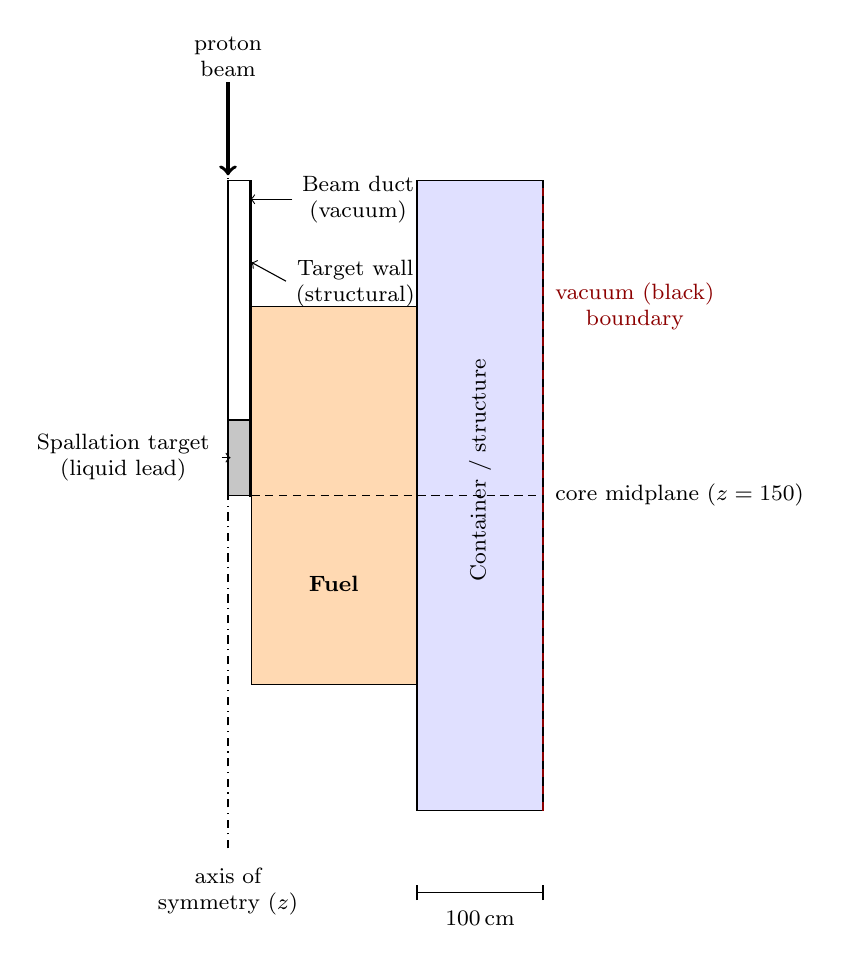
\begin{tikzpicture}[
    x=0.016cm, y=0.016cm,
    font=\footnotesize,
    region/.style={draw=black, line width=0.5pt},
    lead/.style={->, line width=0.4pt},
    lab/.style={align=center}
]

% ---- regions (half r--z section, r >= 0), values from Table~\ref{tab:serpent-geometry} ----
\draw[region, fill=blue!12]   (150,-100) rectangle (250,400); % Container / structure
\draw[region, fill=orange!30] (18.5,0)   rectangle (150,300); % Fuel
\draw[region, fill=gray!70]   (17.5,149) rectangle (18.5,400);% Target wall
\draw[region, fill=white]     (0,210)    rectangle (17.5,400);% Beam duct (void)
\draw[region, fill=gray!45]   (0,150)    rectangle (17.5,210);% Spallation target

% ---- axis of symmetry (= z-axis) ----
\draw[dash dot, line width=0.4pt] (0,-130) -- (0,430);
\node[below, lab] at (0,-138) {axis of\\symmetry ($z$)};

% ---- proton beam ----
\draw[->, line width=1.3pt] (0,478) -- (0,404);
\node[lab] at (0,498) {proton\\beam};

% ---- core midplane ----
\draw[densely dashed, line width=0.4pt] (18.5,150) -- (250,150);
\node[right] at (252,150) {core midplane ($z=150$)};

% ---- vacuum (black) boundary ----
\draw[dashed, line width=0.9pt, red!55!black] (250,-100) -- (250,400);
\node[right, lab, text=red!55!black] at (252,300) {vacuum (black)\\boundary};

% ---- region labels ----
\node[lab] at (84,80) {\textbf{Fuel}};
\node[lab, rotate=90] at (200,170) {Container / structure};

\draw[lead] (-5,180) -- (2,180);
\node[left, lab] at (-7,180) {Spallation target\\(liquid lead)};

\draw[lead] (51,385) -- (17.5,385);
\node[right, lab] at (51,385) {Beam duct\\(vacuum)};

\draw[lead] (46,320) -- (18.5,335);
\node[right, lab] at (46,318) {Target wall\\(structural)};

% ---- radial scale bar ----
\draw[line width=0.5pt] (150,-165) -- (250,-165);
\draw[line width=0.5pt] (150,-171) -- (150,-159);
\draw[line width=0.5pt] (250,-171) -- (250,-159);
\node[below] at (200,-172) {$100\,\mathrm{cm}$};

\end{tikzpicture}
\caption[Serpent \gls{ADS} core geometry.]{To-scale half cross-section
($r$--$z$) of the axisymmetric Serpent \gls{ADS} model, mirrored about the
axis of symmetry. Concentric regions and dimensions are taken from
Table~\ref{tab:serpent-geometry}: a central spallation target filled with
liquid lead on the core midplane, an evacuated beam duct above it, a thin structural target
wall, the surrounding fuel annulus, and the outer container. A vacuum (black)
boundary condition is applied at the outermost surface.}
\label{fig:serpent-geometry}
\end{figure}

\subsubsection{Fuel Compositions and the Case Set}
\label{subsubsec:serpent-materials}

The cases differ in the composition loaded into the fuel region, which is what
makes them a \emph{library} rather than a single run. Each fuel is a transuranic
feed dispersed in a lead matrix. Two representative cases illustrate the range
spanned by the library. In one, the feed is essentially pure minor actinide
dispersed in lead; in another, the feed contains equal masses of plutonium
and minor actinides in lead. These two feeds bracket the
transmutation regimes of interest: a charge containing only minor actinides
maximizes the
minor actinide mass destroyed in each cycle but presents the greatest
reactivity challenge during loading, whereas adding plutonium reduces that
challenge while shifting some of the
destruction burden onto bred and fissioned plutonium. The initial actinide mass
of each case, taken from the day-zero row of its actinide mass table, is the
quantity the archetype's \texttt{capacity} parameter should reproduce, so that a
loaded core matches the case it is compared against.

Each case is depleted along a common ``\(\mathrm{Day}~[\mathrm{d}]\)'' time axis.
The irradiation history is built up from a sequence of chained restart runs: an
initial segment resolves the first fraction of a day with fine steps (for
example, cumulative times of \(0.001\), \(0.1\), \(0.2\), and
\(0.5~\mathrm{d}\)) to capture the rapid early transient in short-lived
fission products, and each subsequent segment reads the binary restart file
written by the previous one and advances the total burnup further (for example,
from \(730\) to \(760~\mathrm{d}\)). Reassembled, these segments give the
continuous nuclide inventory versus irradiation time that the archetype consumes:
an actinide mass table (\texttt{plot\_data\_15\_actinide\_masses\_full.txt} or
\texttt{plot\_data\_06\_actinide\_masses.txt}), a fission product mass table
(\texttt{plot\_data\_14\_fission\_product\_masses.txt}) on the same axis, and a
power history (\texttt{plot\_data\_03\_power\_vs\_time.txt}) used for case
matching. The archetype reads a case's composition at the irradiation time
implied by the cycle length by linearly interpolating these tables along the
day axis, so the resolution of the discharged composition is set by the density
of the Serpent time grid rather than by the \Cyclus time step.

\subsection{Irradiation Event Recording}
\label{subsec:ads-events}

Besides the standard \Cyclus tables, the archetype writes a custom
\texttt{AdsEvents} table so each cycle can be reconstructed without parsing the
full isotopic history. Every row carries the agent ID, time, event type, matched
case, and a mass value (Table~\ref{tab:ads-events}); the matched case is blank on
a load, since matching happens at discharge.

\begin{table}[h!]
    \centering
    \caption{Event types recorded in the \texttt{AdsEvents} output table.}
    \label{tab:ads-events}
    \begin{tabular}{p{0.26\textwidth} p{0.66\textwidth}}
        \toprule
        \textbf{Event} & \textbf{Recorded value} \\
        \midrule
        \texttt{Load} & Mass loaded from feed into the core. \\
        \texttt{Discharge} & Core mass entering the transformation,
                             $M_{\mathrm{in}}$, before Equation~\ref{eq:ads-ratio};
                             the matched case is recorded here. \\
        \texttt{ActinideDestroyed} & Destroyed actinide mass,
                             Equation~\ref{eq:ads-destroyed}. \\
        \texttt{FissionProducts} & Fission product mass in the discharged material. \\
        \texttt{MassDefect} & Mass not retained, $(1-R)\,M_{\mathrm{in}}$. \\
        \bottomrule
    \end{tabular}
\end{table}

The three discharge rows are written only when positive. The
\texttt{ActinideDestroyed} series is the primary performance metric, and its
cumulative sum gives the actinide mass a facility removes from the fuel cycle. With
the standard \Cyclus \texttt{Transactions} and \texttt{ExplicitInventory} tables,
these events close the actinide balance: the actinide initially present equals the
sum destroyed, held in buffers, and resident downstream.

%%%%%%%%%%%%%%%%%%%%%%%%%%%%%%%%%%%%%%%%%%%%%%%%%%%%%%%%%%%%%%%%%%%%%%%%%%%%%%%%%%%%%%%%%%%%%%%%%%%%%%%%%%%%%%%%%%%%%%%%%%%%%%%%%
%%%%%%%%%%%%%%%%%%%%%%%%%%%%%%%%%%%%%%%%%%%%%%%%%%%%%%%%%%%%%%%%%%%%%%%%%%%%%%%%%%%%%%%%%%%%%%%%%%%%%%%%%%%%%%%%%%%%%%%%%%%%%%%%%
%%%%%%%%%%%%%%%%%%%%%%%%%%%%%%%%%%%%%%%%%%%%%%%%%%%%%%%%%%%%%%%%%%%%%%%%%%%%%%%%%%%%%%%%%%%%%%%%%%%%%%%%%%%%%%%%%%%%%%%%%%%%%%%%%

\section{Simulation Scenarios}
\label{sec:simulation-scenarios}

The two archetypes developed in this chapter are exercised in a set of
fuel cycle simulations that share one flowsheet and differ along three axes: the
composition burned in the \gls{ADS}, the length of the simulated horizon, and
whether the discharged material is recycled. Two burner configurations are used,
corresponding to the two representative Serpent cases described in
Section~\ref{subsec:serpent-cases}: a core containing only minor actinides
(ADS~1) and a core containing equal masses of plutonium and minor actinides
(ADS~2). Each configuration is simulated over 30-year and 100-year horizons in
both once-through and recycling modes, resulting in eight simulations.

\subsection{Fuel Cycle Flow}
\label{subsec:scenario-flowsheet}

Every simulation uses the same chain of facilities. The \texttt{us\_inventory}
facility supplies discharged assemblies on the \texttt{snf} commodity under the
\texttt{highest\_minor\_actinide} selection policy
(Section~\ref{subsec:us-inventory-policies}), so that the assemblies richest in
neptunium, americium, and curium are drawn first. A \Cycamore
\texttt{Separations} facility partitions this material: the minor actinides are
routed to the burner feed, while uranium, plutonium (except in ADS~2), and the
fission products fall to a leftover stream sent to a waste \texttt{Sink}. The
\gls{ADS} irradiates the separated feed and discharges the surviving actinides
together with the fission products produced during the cycle. Depending on the
scenario, that discharge is either sent to a \texttt{Sink} (once-through) or
returned to \texttt{Separations} (recycling).

The two burner configurations shape the feed differently. For
ADS~1, which contains only minor actinides, \texttt{Separations} extracts a
single stream of neptunium, americium, and curium at \(99\%\) efficiency and feeds it directly
to the \gls{ADS}. For ADS~2, which contains equal masses of plutonium and minor actinides, the
feed cannot be taken straight from separations: the U.S. inventory holds roughly ten times more
plutonium than minor actinide, so a stream drawn from it is far from an equal
split. \texttt{Separations} therefore produces two streams, one of minor
actinides and one of plutonium, and a \Cycamore \texttt{Mixer} blends them in a
fixed \(0.5/0.5\) mass ratio to reproduce the ADS~2 Serpent feed. The minor
actinide stream limits the feed rate, so surplus plutonium
accumulates in its buffer. This limitation arises from the composition of the
inventory rather than from an imposed modeling constraint.

The separations facilities in these scenarios are idealized material
partitioning models. The simulations assume that an operating reprocessing
system can recover plutonium and the minor actinides into distinct product
streams at the specified \(99\%\) efficiencies. This is an enabling boundary
condition of the analysis rather than a prediction of deployable process
performance. The \textsc{Cycamore} \texttt{Separations} archetype applies
user defined partitioning efficiencies but does not represent process
chemistry, product purity, decontamination factors, plant availability,
secondary waste generation, remote fabrication of actinide bearing fuel,
safeguards, licensing, or the broader policy constraints associated with
commercial reprocessing. The results therefore describe the material flow
performance of the ADS scenarios conditional on such separations
infrastructure being available.

The recycling and once-through modes differ only in the routing of the burner
discharge. In once-through mode the discharge is a terminal waste stream held in
a \texttt{Sink}. In recycling mode it is returned to \texttt{Separations}, which
recovers the surviving minor actinides, and, for ADS~2, plutonium, into fresh
feed, so that actinides make repeated passes through the burner while uranium and
fission products are removed to waste on each pass.

The two routings are shown in Figure~\ref{fig:flowsheet-oncethrough} for the
once-through cycle and Figure~\ref{fig:flowsheet-recycle} for the recycling cycle.

\begin{sidewaysfigure}[h!]
\centering
\resizebox{0.96\linewidth}{!}{%
\begin{tikzpicture}[
    >=Stealth,
    font=\large,
    node distance=2.6cm,
    every path/.style={line width=1.3pt},
    block/.style={
        draw,
        rounded corners,
        minimum width=3.8cm,
        minimum height=2.2cm,
        line width=1.3pt,
        align=center
    },
    blueblock/.style={block, fill=blue!15},
    pinkblock/.style={block, fill=red!10},
    annot/.style={font=\normalsize, align=center},
    keybox/.style={draw, rounded corners=5pt, minimum width=1.4cm,
                   minimum height=0.65cm, line width=0.9pt}
]

\node[blueblock] (inv) {U.S. Inventory\\Facility};
\node[pinkblock, right=of inv] (sep) {Separation\\Facility};
\node[pinkblock, right=of sep] (mix) {Mixer\\Facility};
\node[blueblock, right=of mix] (ads) {ADS\\Facilities};

\node[pinkblock, below=4.3cm of sep] (stor_sep) {Storage\\Facility};
\node[pinkblock, below=4.3cm of ads] (stor_ads) {ADS Storage\\Facility};

\draw[->] (inv) -- node[midway, above, annot]{Assemblies} (sep);

\draw[->] ([yshift=0.45cm]sep.east) -- ([yshift=0.45cm]mix.west)
    node[midway, above, annot]{MAs};
\draw[->] ([yshift=-0.45cm]sep.east) -- ([yshift=-0.45cm]mix.west)
    node[midway, above, annot]{Pu};

\draw[->] (mix) -- node[midway, above, annot]{Material Feed} (ads);

\draw[->] (sep.south) -- (stor_sep.north)
    node[midway, right, annot]{unwanted\\composition};
\draw[->] (ads.south) -- (stor_ads.north)
    node[midway, left, annot]{ADS\\waste};

\draw[->] ([yshift=0.70cm]ads.east) -- ++(4.6cm,0)
    node[midway, above, annot]{Residual Actinides};
\draw[->] (ads.east) -- ++(4.6cm,0)
    node[midway, above, annot]{LLFPs};
\draw[->] ([yshift=-0.70cm]ads.east) -- ++(4.6cm,0)
    node[midway, above, annot]{Other FPs};

% Legend, drawn directly in the same TikZ picture.
\node[keybox, fill=blue!15] (keyblue)
    at ([xshift=3.0cm,yshift=-4.0cm]ads.south east) {};
\node[anchor=west, font=\normalsize]
    at ([xshift=0.25cm]keyblue.east) {Developed in this work};
\node[keybox, fill=red!10, below=0.55cm of keyblue] (keypink) {};
\node[anchor=west, font=\normalsize]
    at ([xshift=0.25cm]keypink.east) {Existing \textsc{Cycamore} archetype};

\end{tikzpicture}%
}
\caption[Once-through fuel cycle flowsheet.]{Conceptual flow for the
once-through fuel cycle. Material from the \gls{STANDARDS}~5.0.1 inventory is
separated, blended when needed, and irradiated in the \gls{ADS}. Separation
waste and \gls{ADS} discharge products follow separate terminal storage paths.
Blue facilities denote archetypes developed for this work, while pink
facilities represent existing \textsc{Cycamore} archetypes.}
\label{fig:flowsheet-oncethrough}
\end{sidewaysfigure}

\begin{sidewaysfigure}[h!]
\centering
\resizebox{0.96\linewidth}{!}{%
\begin{tikzpicture}[
    >=Stealth,
    font=\large,
    node distance=2.6cm,
    every path/.style={line width=1.3pt},
    block/.style={
        draw,
        rounded corners,
        minimum width=3.8cm,
        minimum height=2.2cm,
        line width=1.3pt,
        align=center
    },
    blueblock/.style={block, fill=blue!15},
    pinkblock/.style={block, fill=red!10},
    annot/.style={font=\normalsize, align=center},
    keybox/.style={draw, rounded corners=5pt, minimum width=1.4cm,
                   minimum height=0.65cm, line width=0.9pt}
]

\node[blueblock] (inv) {U.S. Inventory\\Facility};
\node[pinkblock, right=of inv] (sep) {Separation\\Facility};
\node[pinkblock, right=of sep] (mix) {Mixer\\Facility};
\node[blueblock, right=of mix] (ads) {ADS\\Facilities};

\node[pinkblock, below=4.3cm of sep] (stor_sep) {Storage\\Facility};

\draw[->] (inv) -- node[midway, above, annot]{Assemblies} (sep);

\draw[->] ([yshift=0.45cm]sep.east) -- ([yshift=0.45cm]mix.west)
    node[midway, above, annot]{MAs};
\draw[->] ([yshift=-0.45cm]sep.east) -- ([yshift=-0.45cm]mix.west)
    node[midway, above, annot]{Pu};

\draw[->] (mix) -- node[midway, above, annot]{Material Feed} (ads);

\draw[->] (sep.south) -- (stor_sep.north)
    node[midway, right, annot]{unwanted\\composition};

\draw[->, rounded corners=10pt]
    (ads.north) -- ++(0,2.8cm) -| (sep.north)
    node[pos=0.42, above, annot]{Discharged Fuel};

% Legend, drawn directly in the same TikZ picture.
\node[keybox, fill=blue!15] (keyblue)
    at ([xshift=3.0cm,yshift=-4.0cm]ads.south east) {};
\node[anchor=west, font=\normalsize]
    at ([xshift=0.25cm]keyblue.east) {Developed in this work};
\node[keybox, fill=red!10, below=0.55cm of keyblue] (keypink) {};
\node[anchor=west, font=\normalsize]
    at ([xshift=0.25cm]keypink.east) {Existing \textsc{Cycamore} archetype};

\end{tikzpicture}%
}
\caption[Recycling fuel cycle flowsheet.]{Conceptual flow for the closed
(recycling) fuel cycle. Material from the \gls{STANDARDS}~5.0.1 inventory is
separated, blended when needed, and irradiated in the \gls{ADS}; the discharged
fuel is then returned to the separation facility for recovery and reuse. The
unwanted separation stream is sent to storage. Blue facilities denote
archetypes developed for this work, while pink facilities represent existing
\textsc{Cycamore} archetypes.}
\label{fig:flowsheet-recycle}
\end{sidewaysfigure}

All simulations share the remaining settings. Time advances in monthly steps of
\(30.4375~\mathrm{d}\) from a start of January~2025, radioactive decay is
evaluated lazily over the horizon, and explicit inventory tracking is enabled.
The inventory, separations, and mixing facilities each operate at a throughput of
\(250{,}000~\mathrm{kg}\) per step, large enough that material handling does not
throttle the burner.

\subsection{Simulation Runs}
\label{subsec:scenario-runs}

The two burner configurations fix the \gls{ADS} and separations parameters
summarized in Table~\ref{tab:scenario-config}. Each core mass matches the
day-zero actinide mass of the corresponding Serpent case, so a loaded core maps
onto the case it is compared against; the cycle lengths differ by more than the
mass alone, as the large core containing only minor actinides is irradiated
for ten years per cycle while the smaller \(50/50\) core is cycled every two years.

\begin{table}[h!]
    \centering
    \caption{\gls{ADS} and separations configuration for the two burner cases.
    Cycle and refueling times are given in monthly time steps, with the
    equivalent duration in parentheses.}
    \label{tab:scenario-config}
    \begin{tabular}{p{0.30\textwidth} p{0.27\textwidth} p{0.27\textwidth}}
        \hline
        \textbf{Parameter} & \textbf{Case 3 (MA only)} &
        \textbf{Case 4 (50/50 Pu--MA)} \\
        \hline
        Initial core mass  & \(27{,}000~\mathrm{kg}\) & \(4{,}418~\mathrm{kg}\) \\
        Cycle length       & 120 steps (10 yr)       & 24 steps (2 yr) \\
        Refueling time     & 6 steps (6 mo)          & 4 steps (4 mo) \\
        Power level        & \(3000~\mathrm{MW}\)    & \(3000~\mathrm{MW}\) \\
        Separated streams  & Np, Am, Cm              & Np, Am, Cm and Pu \\
        Feed shaping       & Fed directly            &
        \Cycamore \texttt{Mixer}, \(0.5/0.5\) \\
        Serpent case       & \texttt{892\_vt\_ma\_Pb} &
        \texttt{1.3\_vt\_5050\_puma\_Pb} \\
        \hline
    \end{tabular}
\end{table}

Each configuration is simulated over both horizons and in both modes, giving the
eight runs listed in Table~\ref{tab:scenario-runs}. Across most of these runs the
once-through and recycling modes produce nearly identical histories, because the
burner is limited by its cycle duration rather than by feed availability.
Within the horizon, it completes the same number of cores whether or not the discharge is recycled, and the
recovered material only displaces inventory that was still available. The
exception is ADS~1 over the 100-year horizon. Its large core load and ten-year
irradiation cycle draw down the accessible minor actinide inventory, and
recycling allows operation to continue beyond what the once-through supply can
support. The comparison between recycling and once-through in Chapter~\ref{ch:results}
therefore focuses on that pair of runs; for the remaining cases a single
representative run is shown, since the two modes coincide.

\begin{table}[h!]
    \centering
    \caption{Simulation runs. Each burner configuration is run over both
    horizons and in both fuel management modes.}
    \label{tab:scenario-runs}
    \begin{tabular}{c l l l c}
        \hline
        \textbf{Run} & \textbf{Fuel case} & \textbf{Mode} &
        \textbf{Horizon} & \textbf{Steps} \\
        \hline
        1 & MA only      & Once-through & 30 yr  & 360  \\
        2 & MA only      & Recycle      & 30 yr  & 360  \\
        3 & MA only      & Once-through & 100 yr & 1200 \\
        4 & MA only      & Recycle      & 100 yr & 1200 \\
        5 & 50/50 Pu--MA & Once-through & 30 yr  & 360  \\
        6 & 50/50 Pu--MA & Recycle      & 30 yr  & 360  \\
        7 & 50/50 Pu--MA & Once-through & 100 yr & 1200 \\
        8 & 50/50 Pu--MA & Recycle      & 100 yr & 1200 \\
        \hline
    \end{tabular}
\end{table}